\documentclass[a4paper,titlepage,11pt]{article}
\usepackage{a4wide,graphicx,fancyhdr,amsmath,amssymb,color,hyperref}
\usepackage{enumerate}
\usepackage[dvipsnames]{xcolor}
\usepackage{listings}
\usepackage[english]{babel}
\lstloadlanguages{Ruby}
\lstset{%
basicstyle=\ttfamily\color{black},
commentstyle = \ttfamily\color{red},
keywordstyle=\ttfamily\color{blue},
stringstyle=\color{orange}}

%----------------------- Macros and Definitions --------------------------

\setlength\headheight{20pt}
\addtolength\topmargin{-10pt}
\addtolength\footskip{20pt}

\fancypagestyle{plain}{%
	\fancyhf{}
	\fancyfoot[RO,LE]{\sffamily\bfseries\thepage}
	\renewcommand{\headrulewidth}{0pt}
	\renewcommand{\footrulewidth}{1pt}
}


\newcommand{\HRule}{\rule{\linewidth}{0.5mm}}

\newcommand{\uni}{Eindhoven University of Technology}
\newcommand{\fase}{Computer Science and Engineering}
\newcommand{\vak}{Web Information Retrieval \& Data Mining}
\newcommand{\vakcode}{2IMW15 }
\newcommand{\essaytitle}{Neighborhood Safety}
\newcommand{\stad}{Eindhoven}

\pagestyle{fancy}
\fancyhf{}
\fancyhead[R]{\vak}
\fancyhead[L]{\uni}
\fancyfoot[R]{\sffamily\bfseries\thepage}
\fancyfoot[L]{\essaytitle}
\renewcommand{\headrulewidth}{1pt}
\renewcommand{\footrulewidth}{1pt}


\graphicspath{{Images/}}

\author{
	Francis Hoogendijk (0834628) - \texttt{f.c.hoogendijk@student.tue.nl}
	\and
	Bram Kohl (0746107) - \texttt{b.j.e.kohl@student.tue.nl}
	\and
	Guus van Lankveld (0629468) - \texttt{g.v.lankveld@student.tue.nl}
	\and
	Jasper Selman (0741516) - \texttt{j.w.m.selman@student.tue.nl}
	\and
	Ramon de Vaan (0758873) - \texttt{r.d.vaan@student.tue.nl}
	\and
	Bart van Wezel (0740608) - \texttt{b.j.p.a.v.wezel@student.tue.nl}
}
\begin{document}
	
	\begin{titlepage}
	\begin{center}

% Upper part of the page
		
\includegraphics[width=0.15\textwidth]{Images/tuelogo}\\[1cm]

		\textsc{\LARGE \uni}\\[0.2cm]

		\textsc{\fase}\\[1.6cm]

        \textsc{\LARGE \vak}\\[0.5cm]

% Title
\HRule \\[0.4cm]
{ \huge \bfseries \essaytitle}\\[0.4cm]

\HRule \\[1.5cm]

% Author and supervisor
	\emph{Group TODO:}\\
    \begin{tabular}{l l l}
	Francis \textsc{Hoogendijk} & 0834628 & \href{mailto:f.c.hoogendijk@student.tue.nl}{\texttt{f.c.hoogendijk@student.tue.nl}}\\
	Bram \textsc{Kohl} & 0746107 & \href{mailto:b.j.e.kohl@student.tue.nl}{\texttt{b.j.e.kohl@student.tue.nl}}\\
	Guus \textsc{van Lankveld} & 0629468 & \href{mailto:g.v.lankveld@student.tue.nl}{\texttt{g.v.lankveld@student.tue.nl}}\\
	Jasper \textsc{Selman} & 0741516 & \href{mailto:j.w.m.selman@student.tue.nl}{\texttt{j.w.m.selman@student.tue.nl}}\\
	Ramon \textsc{de Vaan} & 0758873 & \href{mailto:r.d.vaan@student.tue.nl}{\texttt{r.d.vaan@student.tue.nl}}\\
	Bart \textsc{van Wezel} & TODO & \href{mailto:r.d.vaan@student.tue.nl}{\texttt{TODO}}
    \end{tabular}
		\vfill

% Bottom of the page
		{\large \today} \\
		\stad

	\end{center}
\end{titlepage} 
	
	\section{Introduction}
\subsection*{Project Idea}
Every now and then people wonder if the neighborhood they are living in is still safe and what is happening in their neighborhood. 
We got a solution for this. We want to create a program in which people can search for their (home)city and see what is happening. They receive a news feed of articles concerning their neighborhood and a list (visualized by circles on a map) of events in which the emergency services were involved. To retrieve these, we will use the P2000 system used in the Netherlands. The news feed will either be extracted from local news sites, Twitter or both. This is yet to be determined. 

\subsection*{Data}
The data that we will use for our project will be extracted from several different sources. These sources are yet to be determined but the data can already be cut in two clear distinct parts. One part consists of data that we will extract out of the P2000 system used in the Netherlands. This system contains notifications of events where emergency services were needed. There are several sites which can be used to retrieve this data. 
The second part contains the news feed or Twitter data we want to show when people are searching for their city. We do not yet know whether we want to use Twitter data, local newsfeeds, or both as we do not know how hard it is to retrieve data from local news sites and we do not know how much noise Twitter will contain.
\subsection*{Goals}
The goals in this project are as follows. At first we want to create a basic system where people can search for a city and a timeframe. When they do that we want to visualize a map of the Netherlands zoomed in on that city. The map contains several colored dots. Every dot will represent an event in which the emergency services were involved. We want to use different colors for different services (police, fire department and ambulance) and let the size of the circle depend on how serious the event was. This is the basic outline of the project which has to work for 100$\%$. Furthermore, we want to be able to click on the circles which will trigger a pop up to appear with local, related news to the event. This news is extracted from either Twitter or local news sites as mentioned before. Another feature we would like to implement is to use classifications in the search. For example I would like to only see events which involved murder or robbery. We do not know how hard this is, so we see it as an optional feature.
\subsection*{Tasks}
The IR and ML tasks are divided such that one person contributes at at least one of each. The tasks are shown in \autoref{tab:tasks}

\begin{table}[!h]
\begin{center}
\centering

\begin{tabular}{| l| l | l| l |}
\hline
                   & {\bf Student ID} & {\bf Information Retrieval}                                                            & {\bf Machine Learning}                                                                       \\
\hline
Francis Hoogendijk & 0834628             & Collect P2000 notifications                                                            & \begin{tabular}[c]{@{}l@{}}Retrieve keywords from \\ P2000 notifications\end{tabular}     \\
\hline
Bram Kohl          & 0746107          & Indexing of notifications                                                              & Cluster notifications                                                                       \\
\hline
Guus van Lankveld      & 0629468          & \begin{tabular}[c]{@{}l@{}}Collect news feed / \\ twitter data\end{tabular}            & \begin{tabular}[c]{@{}l@{}}Extract locations from \\ news feed / twitter data\end{tabular}   \\
\hline
Jasper Selman      & 0741516          & \begin{tabular}[c]{@{}l@{}}Language detection \& \\ spell check\end{tabular}           & \begin{tabular}[c]{@{}l@{}}Classify news feed / twitter \\ data\end{tabular}                 \\
\hline
Ramon de Vaan      & 0758873          & \begin{tabular}[c]{@{}l@{}}Create database of P2000 \\ notification codes\end{tabular} & Association analyzer                                                                         \\
\hline
Bart van Wezel     & 0740608            & Indexing of news feed / twitter data                                                   & Classification of P2000 notifications                                                                \\
\hline

\end{tabular}
\caption{Tasks}
\label{tab:tasks}
\end{center}
\end{table}

	\newpage
\section{Architecture}
TODO write text.

\begin{figure}[h!]
  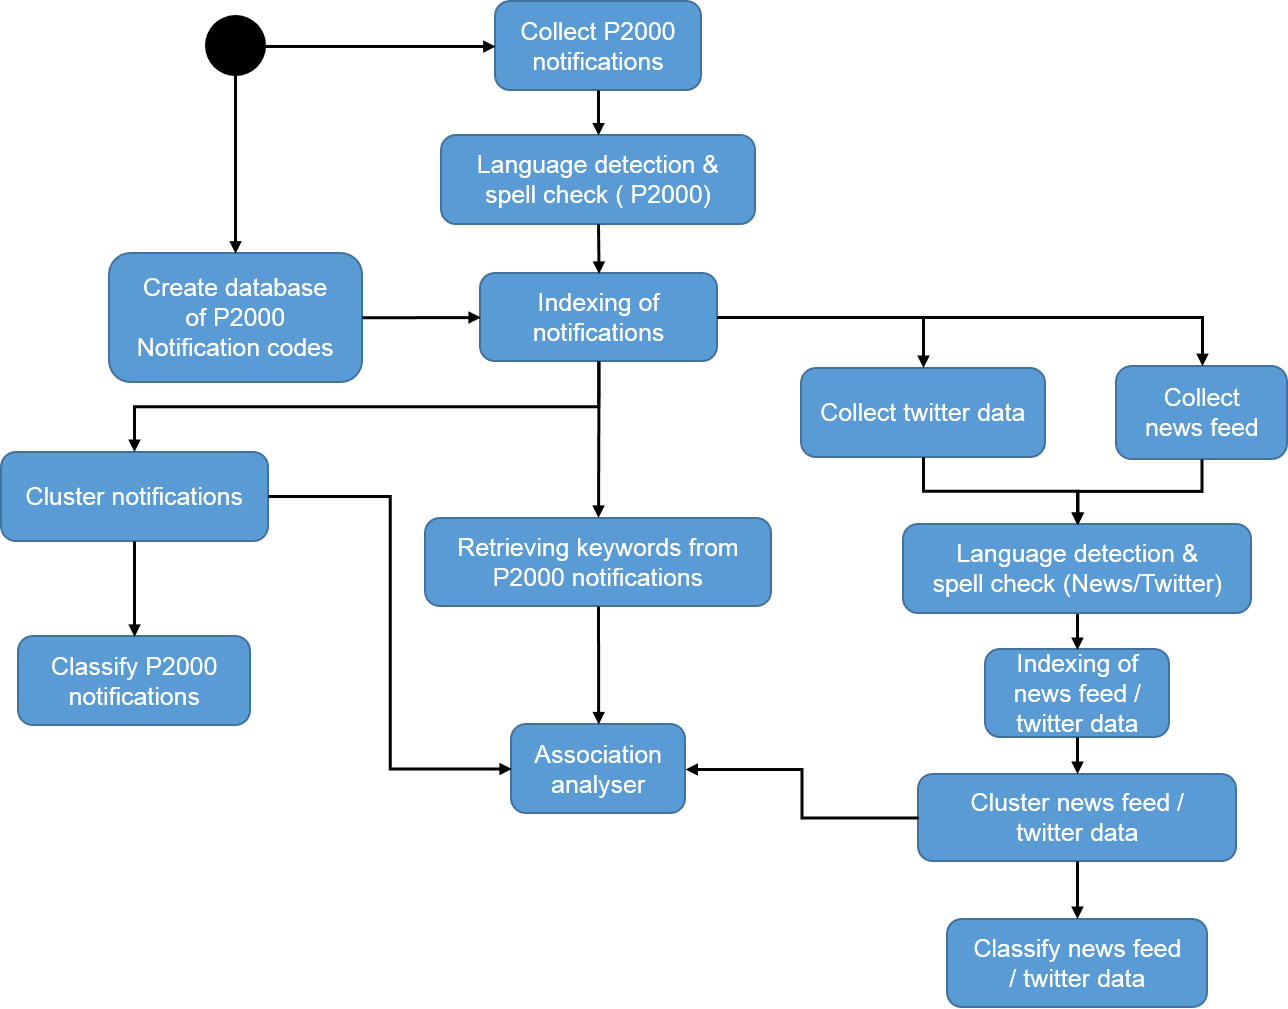
\includegraphics[width=0.9\linewidth]{Architecture.png}
  \caption{Program architecture}
  \label{fig:Architecture}
\end{figure}
	
	\newpage
	\section{Information Retrieval}
	\subsection{Collect P2000 notifications}
\textbf{Name:} Francis Hoogendijk \indent \textbf{StudentNumber:} 0834628

\subsubsection*{Motivation}
As described in the introduction, the program that we want to build should show events which required emergency services in a specified neighbourhood. For this we plan to use notifications of the Dutch P2000 system. These notifications can be accessed through several different websites and contain timestamped information about which emergency response team is required, where they should go and sometimes other information. In order to process this information, we first need to extract the notifications from one or more sources (to be determined). To do this, we intend to use a crawler that will extract the notifications' content from the website(s). Since the P2000 system is continually operational, the crawler should frequently check for new notifications (the exact frequency still needs to be determined). 

\subsubsection*{Approach}
The crawler will be made so that it extracts P2000 notifications from a given source (or sources). The notifications may go back several years, so an endpoint (starting date) will have to be determined to limit the amount of data to be collected. Once all available notifications up to the present time are collected, the crawler should frequently check for new notification and add them to the collection if necessary. The implementation of the crawler still needs to be determined based on the choice of websites to extract from and their content. Also available API's that are of use (if any) will be utilized. The crawler will only collect the raw notification data, which will later be indexed and processed to extract relevant information. 

\subsubsection*{Evaluation}
The evaluation of the crawler will be done mainly by manually checking the collected data, and the ability for it to update its collection with new P2000 notifications.
	\subsection{Indexing of notifications}
\textbf{Name:} Bram Kohl \indent \textbf{StudentNumber:} 0746107

\subsubsection*{Motivation}
When the P2000 data has been retrieved, it is just raw data. There is no clear structure in it yet and as such, it has to be indexed, so we can easily use it later on. For example, in order to be able to associate the P2000 notifications with the messages from the news feed and twitter data, we want to be able to easily and quickly obtain information about the notifications. Information like the date and time the emergency service was called, which emergency service was called (fire department, police department or ambulance), with what urgence the emergency service was called, where the incident happened and suchlike. So what we want to do is extract a lot of information from the raw (html) data and possibly from some other sources (e.g. get name of town from postal code). We want to store that information in a structured and easily accessible way.
\subsubsection*{Approach}
The indexing part kicks in when the raw data has already been retrieved. This data contains html code which has a structure we can work with. It consists of a table with a few rows per notification. Using the rows and columns of this table we can extract the date and time the emergency service was called, the type of emergency service it concerns and the region the incident happened (25 possible regions, so about 2 regions per province). Furthermore, if there are capcodes present (codes which indicate the region and type of emergency service) we extract those as well.\\

Furthermore, we extract a table field which contains a message for the notification. This message often contains a postal code and/or the name of a town. As we would like to know the location more specific than just the region, we try to extract this information from the message.
The postal code can be extracted using the structure of a postal code (4 numbers and two letters, with an optional space in between). We do this using a regular expression.\\

The name of a town can be obtained in two ways. If we find a postal code in the message, we obtain it using the api at \url{http://www.postcodeapi.nu}. This is the most reliable way of the two. If we don't have a postal code, we attempt to extract it from the P2000 message using a database of towns in the Netherlands. We created this database from a list of 5712 towns that we found online (\url{http://home.kpn.nl/pagklein/almanak.html}). We check for each town whether it occurs in the message as a whole word and if it does, we store the town. If we detect multiple towns, we store all of them so the association analyzer can take all of them into account.\\

When we have isolated and transformed all the data we need, we store it in SQL database tables with a clear structure, so we can later easily access the data. We create indexes on this database on several fields (e.g. date and time and postal code) to speed up future search queries.
\subsubsection*{Evaluation}
The indexing of notifications will be evaluated by manually checking the resulting data in the database, to see whether the data has been split up properly, and by running queries and testing how long they take to see whether the indexes are working properly. These manual tests showed that (in the end) everything works as expected.
	\subsection{TODO GUUS}
\subsubsection*{Name part}
\textbf{Name:} TODO \indent \textbf{StudentNumber:} TODO

\subsubsection*{Motivation}

\subsubsection*{Approach}

\subsubsection*{Evaluation }
	\subsection{Language detection \& spell check}
\textbf{Name:} Jasper Selman \indent \textbf{StudentNumber:} 0741516

\subsubsection*{Motivation}
When retrieving data from the internet there is a problem which every programmer faces: the incapability of the human being to agree on one single set of unambiguous rules to write words and the ability to actually write according to these rules. On most sites there are a lot of spelling errors made and words are written in a different way because the grammatical and spelling rules let him do that. \\
When you want to index the data retrieved you do not want that two words who only differ in some spelling error are indexed different from each other. That's why we need a spell check. We also do not want the same words in different languages to differ from each other. When we focus on local news sites this will not be a problem, but if we use Twitter data this might be a problem.

\subsubsection*{Approach}
At the start we had to discuss what we really wanted to enhance, since there are a lot of possibilities to improve and or check texts. We agreed on a couple of things. Firstly we thought that language detection would not contribute a lot to our project. This is because the P2000 system and the local news sites are ensured to be in Dutch and it is very likely that the greater part of the Twitter data is also in Dutch. Next to that we also did not know how hard it was to detect a language, that is why we decided to give this detection a low priority and only try to implement it when we finished the rest. \\
We also concluded that it was enough to tokenize and stem the twitter/news data. This would improve the text significantly, because words who are very similar to each other such as werken, werkt and werk (which are Dutch words for working). All these words have the same stem. I have also searched for possibilities to fix real spelling mistakes such as aple instead of apple, but I found that there are certain tools who can do this for a small amount of input (such as a query), but not for a whole text file. So the focus was on tokenization and stemming.\\
After a bit of research I found a whole bunch of tools who supported either tokenization or stemming, but unfortunately not both. Happily we also found one tool which supported both. This tool is called Elasticsearch TODO REFERENCE. This is a tool where it is possible to store data on our own server (news and twitter data) and edit this data by applying several "analyzers" on them. These analyzers worked in a way such that you could add filters, like stemmers, and tokenizers to an analyzer which is saved. After you created the analyzer you could do a call to this analyzer and give it text as input. So the goal was now to create the analyzer we wanted and to make sure that it runs on our server. \\
I immediately noticed that there were a lot of options in Elasticsearch to modify text, but we were very limited due to the constraint that our text was in Dutch. There were in fact two good options for stemming and only one option as a tokenizer. As tokenizer we used a simple white space tokenizer. I tested a bunch of other tokenizers which were available but they did not give significant better results than the white space tokenizer and in combination with how easy to use the normal tokenizer is, we picked that one (punctuations were handled by the stemmers). \\
As a stemmer we had the possibility between a Hunspell stemmer, which uses a dictionary, and the Porter Snowball stemmer, which was based on an algorithm. After some searching we found a Dutch dictionary for the first stemmer, but we still decided to create the Snowball stemmer, because its results were better and we were not dependent on the quality of the dictionary. As a backup we also created a Hunspell analyzer. Both the analyzers can be found in TODO REFERENCE TOEVOEGEN VOOR ANALZYERS.\\
I have also thought about adding phoenetic search, since a lot of the spelling errors in Dutch are mixing up whether a word should end with d or t or dt or use au instead of ou or ei instead of ij. All these variations do sound the same however, so it makes sense to use phoenetic search. Only the problem was almost all phoenetic search algorithms support English and we needed support for Dutch. I was not able to find an algorithm which supports Dutch, so unfortunately we were not able to make use of this type of search.

\subsubsection*{Evaluation $\&$ Possible Improvements }
The evaluation of the language detector can be done manually, since we can immediately see if that worked, if a lot of the words are corrected we might have detected the wrong language. To evaluate the spelling check is bit more tricky I guess. One thing that comes to my mind is to first index the retrieved data without a spelling check and after that do the same with a spelling check. This will be done using small text documents like news feed. Using this small documents we can manually check if the spelling corrector, did his work.
TODO: BREIDT DIT UIT EN IMPROVE DIT NA TESTEN

	\subsection{TODO RAMON}
\subsubsection*{Name part}
\textbf{Name:} TODO \indent \textbf{StudentNumber:} TODO

\subsubsection*{Motivation}

\subsubsection*{Approach}

\subsubsection*{Evaluation }
	\subsection{Indexing of news feed / twitter data   }
\textbf{Bart van Wezel}  \indent \textbf{0740608} 

\subsubsection*{Motivation}
The indexing should happen after the Language detection \& spell check is applied. This way we know that the input data is mostly correct.  The collected data should be stored in a efficient way, such that queries can be executed on the data. This should be done in an efficient way, which can be done with indexing the collected data. 

\subsubsection*{Approach}
How the data is going to be indexed still depends on the queries needed by the machine learning components. Especially the components: Classify news feed/twitter data and the Association analyser. If those components need phrase queries , we create a Positional index.  A positional index is now commonly used, because of the power and usefulness of phrase and proximity queries. However if no phrase queries are needed, a simple Inverted index construction will be used. Here multiple query optimization techniques will be applied. For example the merge method with skip pointers could be implemented. 

\subsubsection*{Evaluation }
The evaluation of the Indexing of news feed / twitter data component, can be done by executing queries on the indexed data. Then we can compare those results with actually searching the documents for the same query. Actually searching the documents can be done automatically, but will probably take some time. For testing the queries this is not a real problem, because the tests can be executed before the indexing is going to be used. The tests are probably secure, because actually searching the original documents gives the exact desired outcome. This outcome should match the outcome of the queries. However we will probably only execute this tests just after indexing, because storing all the original documents will occupy a lot of space. 

	
	\section{Machine Learning}
	\subsection{Graphical User Interface and Classification of tweets}
\textbf{Name:} Francis Hoogendijk  \indent \textbf{StudentNumber:} 0834628

Initially, my ML task was to extract keywords from P2000 notifications. This seemed a valid task when distributing at the start of the course, but later we realized that we were not even using keywords. The classification and association tasks did not have a use for keywords either. Besides, the extraction was complex due to the way P2000 notifications are written; They are written in Dutch (which makes finding an extraction tool difficult) and have little resemblance to natural speech. \\

Because of this, my task was changed to assist in the classification tasks, which required help on training the classifier for tweets, as it is a time consuming task. Besides that, a GUI was required to present our combined work in a visually pleasing way.

\subsubsection*{Motivation}
\textbf{Classification of tweets}\\
The classification of twitter messages is required to facilitate association analysis between P2000 notifications and tweets. Tweets by definition short text messages.\\

\textbf{Graphical User Interface}\\
To present people the functionality of this system, a Graphical User Interface (GUI) is a must. People should be able to search for their city and view their neighbourhood on a map and be able to click on items they find relevant. 
 
\subsubsection*{Approach}
\textbf{Classification of tweets}\\
For classifying the twitter messages, the same Ruby library as used for classifying P2000 notifications and news feed was used (\autoref{app:classifier}). The Na\"{i}ve Bayes classifier was chosen for the twitter messages, since TF.IDF is regarded as inferior for short documents, as they can contain a lot of noise. From the gathered tweets in the database, a sample set was chosen and their content was labeled and used to train the classifier analogue to the training of the other classification tasks. Only relevant training words were added by removing irrelevant words from tweets such as names of towns or places.\\

The tweets were divided in the classes: \emph{Police}, \emph{Ambulance},\emph{Firefighters}, \emph{Fire}, \emph{Accident}, \emph{Crime},  and \emph{Other}. The Other class has some subdivisions to reduce its size, which would otherwise give it too much weight. This is necessary because there are a lot of irrelevant tweets. Also the tweets relating to firefighters became a large class, so it was split into tweets relating to actual fires, and other tasks for which firefighters are also called.\\

The above mentioned approaches could be used because previous classification tasks were already done on P2000 notifications and the news feed. This facilitated me to only focus on the time consuming part of creating a training data set and getting a good sense of the classifiers.

\textbf{Graphical User Interface}\\
Due to my limited programming experience, I chose to use Java's Swing to build the GUI, combined with the JxBrowser library from TeamDev. This library allows the embedding of a chromium-based element in Swing applications. These elements could then load HTML files containing JavaScript code for dynamic and interactive layouts of the pages. The JxBrowser library also facilitates the possibility to perform function calls between the Java application and the HTML files (and back too).\\ 

The required interactive components of the GUI flowed from our description of the system; it needs a search box to have users enter their city, and a display to show them a map of that city. The map can show the locations of the P2000 notifications based on the extracted textual location information, and passing that through a geocoding API to extract coordinates. Also, since there may be many P2000 notifications, the user must specify a date to view only data of that specific date. This is implemented using a slider, as it intuitively visualizes a timeline on which one can go back. \\
Besides the P2000 notifications, the system has to show the possibly related news items and tweets. For this purpose, the GUI was designed as a full-screen 
application split in two halves. The left half shows the map using the Google maps API with obove it a search box and button accompanied by a time slider. The right half is split in a top and bottom quarter for related news items and tweets respectively. \\

Using the system, a user queries their town of interest on a date of interest. The user can then click markers that have appeared on the map which represent the locations of P2000 notifications. The markers are color coded red for firefighters, blue for police and yellow for ambulance. Upon clicking a marker, related P2000 notifications (from the P2000 notification clustering) are shown in a pop-up info window, and the related news items and tweets are extracted from the database and shown on the right half of the screen. \\


\subsubsection*{Evaluation $\&$ Possible Improvements}
\textbf{Classification of tweets}\\
The classifier was evaluated analogue to the method used to classify news and P2000 notifications. This was done by giving the classifier unlabeled data and comparing its outcome with labels that we deemed fitting. If it labeled many tweets incorrectly, the training set was increased in size. This process was repeated until reaching desired behavior. In this case, desired was to allow for false negatives, but prevent false positives. Since the labels or classes are used in the association analysis, this would reduce the amount of irrelevant tweets as much as possible at the cost of maybe missing some relevant ones. This would give the user confidence in the suggested associations, whereas viewing irrelevant suggestions repeatedly quickly will reduce the users' confidence in the system.

\textbf{Graphical User Interface}\\
The evaluation of the GUI was done manually by looking for associations of news items and tweets in the database. Then by querying the corresponding town, clicking the P2000 notification on the map and viewing the correct items appearing, the GUI was deemed functional. \\

Performance of the GUI might still be improved, as it now loads the associated news and tweets upon clicking them on the map. Also the clustered P2000 notifications might be retrieved in a more efficient manner than currently implemented. 
	\subsection{Cluster notifications}
\textbf{Name:} Bram Kohl \indent \textbf{StudentNumber:} 0746107

\subsubsection*{Motivation}
When an incident that requires emergency services happens, there are often multiple notifications in the P2000 system concerning that single incident. Take for example a car accident. This often requires the fire department to cut open cars, the police department to organize the other traffic and one or more ambulances to take care of the passengers of the cars involved in the accident. These all show up as separate notifications in the P2000 system. As we want to be able to associate the P2000 notifications with news messages and/or twitter messages, we would like to combine these notifications that belong to the same incident.
\subsubsection*{Approach}
As input, we have many P2000 notifications and as output we would like to know which P2000 notifications belong together. In order to do this, we run through the database and for each P2000 notification, we check for other notifications that came in around the same time this one did (with a certain error, for example 2 hours) and that went to the same address. We assume that these notifications belong to the same incident.\\\\
We might extend this by checking whether the addresses of two notifications are close to each other when they do not exactly match (but the time does match), and similarly whether it concerns the same incident when the calls are further apart but address does match. We could determine a probability for this by looking for similar words in the message provided with the call.
\subsubsection*{Evaluation}
The clustering of notifications will be evaluated manually, by searching for a few P2000 notifications that should be matched together (these occur rather frequently, so that should not be too hard) and checking whether they are properly indicated as belonging together. Furthermore, we will check whether messages that should not be matched are not indicated as belonging together as well.
	\subsection{Associate P2000 notifications with news articles}
\textbf{Name:}  Guus van Lankveld \indent \textbf{StudentNumber:} 0629468

\subsubsection*{Motivation and relation to project}
Our project attempts to find relevant news articles for certain P2000 notifications, which are linked to events in a specified neighborhood. To determine the relevancy of news articles, P2000 notifications need to be associated with news articles that are relevant to these notification. It is assumed that a certain amount of preprocessing of notifications and articles is done by other modules of the retrieval system, these processed articles have the following properties:
\begin{enumerate}
\item Each notification has a date, a number of labels and possibly a location.
\item Each news article has a date and a number of labels.
\end{enumerate}
Using a simple modified version of association rule learning, the relations between each group of P2000 notifications and group of news articles can be determined.  

\subsubsection*{Approach}
The assumption is made that the other parts of the system have already classified both P2000 notifications and news articles and that these labels are correct. A simple matching scheme is implemented that matches notifications according to their labels and assigned date and location tags. The labels and tags of each matching notification and article can be converted to an association rule corresponding to the relation between these items. For each association rule, a number of metrics can be computed (e.g. support, confidence) which can be used to create a ranking that indicates the strength of the association. This data can be used by other parts of the system to display the most relevant news articles.

\subsubsection*{Implementation and Evaluation }
An custom algorithm is used to build the association list. The input of the algorithm are a list of classified P2000 notification data and a list of classified news article data. A few remarks about the data which is outputted by both the notification classifier and the news classifier are (by examining the results outputted by those parts):
\begin{enumerate}
\item Every P2000 notification and news article has an id number and primary label
\item Most P2000 notifications have a second label. 
\item Most P2000 notifications have a location tag.
\item All news articles have a location tags.
\end{enumerate}

Some example data that the associator will use is illustrated in \autoref{tab:p2000data} and \autoref{tab:newsData}. 
\begin{table}[]
\centering
\begin{tabular}{|l|l|l|l|l|}
\hline
\textbf{notification} & \textbf{label} & \textbf{sublabel} & \textbf{date} & \textbf{town} \\ \hline
16129                 & Ambulance      & Accident          &               & Amsterdam     \\ \hline
34537                 & Police         & Crime             & 16-10-2015    & Eindhoven     \\ \hline
68778                 & Fire dept.     &                   & 19-10-2015    &               \\ \hline
\end{tabular}
\caption{Example labeled P2000 data}
\label{tab:p2000data}
\end{table}

\begin{table}[]
\centering
\begin{tabular}{|l|l|l|l|}
\hline
\textbf{news\_id} & \textbf{label} & \textbf{date} & \textbf{location} \\ \hline
24                & Police         &  16-10-2015             & Eindhoven         \\ \hline
76                & Fire dept.     & 16-10-2015    & Arnhem         \\ \hline
89                & Ambulance      & 19-10-2015    & Amsterdam            \\ \hline
\end{tabular}
\caption{Example labeled news article data}
\label{tab:newsData}
\end{table}

The algorithm to build association rules works as follows:
\begin{enumerate}
\item Compare each P2000 $p$ notification and news article $n$ with each other and create an association rule if both of the following conditions hold: 
	\begin{itemize}[noitemsep]
	\item The location tag is the same for both the P2000 notification and the news article
	\item At least one label that occurs in $p$ also occurs in $n$: $labels(p) \cap labels(n) \not= \emptyset$
	\end{itemize}
\item Compute the support and confidence of both sides of the association rule, as well as the lift.
\item Compute a score for each rule:
\end{enumerate}


\subsection{Improvements and future work}
	\subsection{Classify news feed / Twitter data}
\textbf{Name:} Jasper Selman \indent \textbf{StudentNumber:} 0741516

\subsubsection*{Motivation}
People often want to know what is happening in the neighbourhood, but they do not want to know every little thing that is happening.
They are only interested in certain type of news. This is why we want to classify the news feed / Twitter data such that people can choose from a set of subjects. For example people only want news about events which involved an ambulance. 

\subsubsection*{Approach}
The real approach to do this is yet to be researched and determined, but an initial idea is to first create a set of subjects we offer the user to choose from. For every possibility in that set we should create a set of relevant similar words. Next to that we should classify every news item with some kind of algorithm such that if one of the words of the set for a search term occurs enough (the amount has to be determined) in the news item, then the item is classified for that search term.

\subsubsection*{Evaluation }
This will be checked manually, because it is very easy to check, when you choose a subject, if the resulting news feed shown indeed involved the subject or that also other news is shown.

	\subsection{TODO RAMON}
\subsubsection*{Name part}
\textbf{Name:} TODO \indent \textbf{StudentNumber:} TODO

\subsubsection*{Motivation}

\subsubsection*{Approach}

\subsubsection*{Evaluation }
	\subsection{Classification of P2000 notifications }
\textbf{Name:} Bart van Wezel \indent \textbf{StudentNumber:} 0740608

\subsubsection*{Motivation}
Not all P2000 notification are really clear. A example of an notification can be: \\ 
10-09-15	16:05:06	Ambulance	Midden- en West Brabant	B1 5011ME X : Mahlerstraat X Tilburg 67893  \\
This notification is not really interesting to see, because when you get to see such a notification you probably have no idea what happened. 
With a bit of research you can find that B1 means ordered transport. For example from the hospital to a nursing home. 
We are going to try to classify the P2000 notifications, such that we can get a clear classification for each P2000 notification.
This way we can make the program more useful for a general public. 

\subsubsection*{Approach}
To classify the P2000 notifications, we will try to find a main classification and a sub-classification. 
A main classification could be some issue with the train. 
The sub classification could be fire on the track. 
To find those classifications we have to write a algorithm that tries to classifies the notifications. 
Those classification can be done with a list of all abbreviations and use this list to determine which main classifications and sub classifications there should be. 

\subsubsection*{Evaluation }
We can evaluate this part by manually classifying  multiple P2000 notifications and then apply the algorithm to those P2000 notifications.
When the result of the algorithm is the same as the manually classified notifications, we know that the algorithm probably works correctly.

	\section{Project Evaluation}
Since there are a lot of P2000 notifications, we can create a test data set. 
In this data set we will manually classify the notifications and manually create clusters. 
Furthermore, we are manually going to search news web pages and tweets from twitter.
We will classify those news web pages and tweets from twitter. 
Then we can run the whole project on this data set  and check if the ML tasks will produce the same output.

The IR tasks can be evaluated by running queries on the database. 
Then we will check if those queries give the desired results, by manually checking the data set for those queries.
TODO voeg hier een link naar de code toe

	\newpage

	\begin{appendix}
	\section{Appendix Language Analysis in Elasticsearch} \label{app:irjasper}
In this part we will explain how you should install Elasticsearch on your own computer/server and what need to be done to run the analyzers created for the language analysis.
\begin{itemize}
\item The first step is to download Elasticsearch from: \url{ https://www.elastic.co/}.
\item Start the Elasticsearch filer by running the bat file in the bin directory.
\item From the root of the Elasticsearch folder run the command: \\
\texttt{bin/plugin -i elasticsearch/marvel/latest}. This should give an interface to work with Elasticsearch.
\item Now in the config directory open the file \texttt{elasticsearch.yml} and add the following two properties to the file: 
\texttt{indices.analysis.hunspell.dictionary.ignore$\_$case: true} and \texttt{indices.analysis.hunspell.dictionary.strict$\_$affix$\_$parsing: true}. 
\item In the same directory create a new folder called \texttt{hunspell} and put the Dutch dictionary in it. This dictionary , named \texttt{n$\_$NL}, can be downloaded from \\
\url{http://download.services.openoffice.org/contrib/dictionaries/}.
\item Unpack it in the \texttt{hunspell} directory and make sure that the path structure is\\
 \texttt{config/hunspell/nl$\_$NL/}.
\item Now go to the url \url{http://localhost:9200/_plugin/marvel/sense/index.html}.
\item Now in the left side put the two analyzers provided on the next page (simple copy and paste would work).
\item When you hover over the line with \texttt{put} on it, you see a green triangle. When you click it you create the new analyzer. This has to be done for each of the two analyzers.
\item Now when you put a GET request on the left side you are able to analyze text. An example GET request is:\\
\texttt{GET $/$snowball$/$$\_$analyze?analyzer$=$my$\_$analyzer }\\
\texttt{$\{$Dit voorbeeld laat zien hoe Nederlandse analyzers werken$\}$ }.\\
When you replace \texttt{snowball} by \texttt{hunspell} and \texttt{my$\_$analyzer} by \texttt{nl$\_$NL} you can apply the Hunspell analyzer to the request. 
\end{itemize}
\newpage

\noindent\texttt{PUT $/$snowball} \\
\texttt{$\{$}\\
\indent \texttt{"index" : $\{$}\\
\indent \indent \texttt{"analysis" : $\{$}\\
\indent \indent \indent \texttt{"analyzer" : $\{$}\\
\indent \indent \indent \indent \texttt{"my$\_$analyzer" : $\{$}\\
\indent \indent \indent \indent \indent \texttt{"tokenizer" : "standard",}\\
\indent \indent \indent \indent \indent \texttt{"filter" : ["standard", "lowercase", "my$\_$snow"]}\\
\indent \indent \indent \indent \texttt{$\}$}\\
\indent \indent \indent \texttt{$\}$,}\\
\indent \indent \indent \texttt{"filter" : $\{$}\\
\indent \indent \indent \indent \texttt{"my$\_$snow" : $\{$}\\
\indent \indent \indent \indent \indent \texttt{"type" : "snowball",}\\
\indent \indent \indent \indent \indent \texttt{"language" : "Dutch"}\\
\indent \indent \indent \indent \texttt{$\}$}\\
\indent \indent \indent \texttt{$\}$}\\
\indent \indent \texttt{$\}$}\\
\indent \texttt{$\}$}\\
\texttt{$\}$}\\
\\
\noindent\texttt{PUT $/$hunspell} \\
\texttt{$\{$}\\
\indent \texttt{"settings" : $\{$}\\
\indent \indent \texttt{"analysis" : $\{$}\\
\indent \indent \indent \texttt{"filter" : $\{$}\\
\indent \indent \indent \indent \texttt{"nl$\_$NL" : $\{$}\\
\indent \indent \indent \indent \indent \texttt{"type" : "hunspell",}\\
\indent \indent \indent \indent \indent \texttt{"language" : "nl$\_$NL"]}\\
\indent \indent \indent \indent \texttt{$\}$}\\
\indent \indent \indent \texttt{$\}$,}\\
\indent \indent \indent \texttt{"analyzer" : $\{$}\\
\indent \indent \indent \indent \texttt{"nl$\_$NL" : $\{$}\\
\indent \indent \indent \indent \indent \texttt{"tokenizer" : "standard",}\\
\indent \indent \indent \indent \indent \texttt{"filter" : ["lowercase", "nl$\_$NL"]}\\
\indent \indent \indent \indent \texttt{$\}$}\\
\indent \indent \indent \texttt{$\}$}\\
\indent \indent \texttt{$\}$}\\
\indent \texttt{$\}$}\\
\texttt{$\}$}\\
\clearpage

	\newpage
	\section{Appendix Ruby Classifier} \label{app:classifier}

We used a Ruby library, so before installing the library we have to install Ruby and Rubygems.
This can be done on an Ubuntu 14.04 server by the following commands. 
\begin{lstlisting}[frame=single]
sudo apt-get install ruby
sudo apt-get install rubygems-integration
\end{lstlisting}
For installing Ruby somewhere else, we recommend looking at: \url{ https://www.ruby-lang.org/en/} for more information to install Ruby on another operating system. \\
\textbf{Stuff-Classifier:} \\
A library for classifying text into multiple categories.
It currently provides two different classifiers namely: 
\begin{enumerate}
\item A Naive Bayes classifier
\item A classifier based on TF-IDF weights
\end{enumerate}
It can be installed with the following command: 
\begin{lstlisting}[frame=single]
gem install stuff-classifier
\end{lstlisting}
The classifier can be used like this:

\begin{lstlisting}[language=Ruby]
require 'stuff-classifier'

cls = StuffClassifier::Bayes.new("Cats or Dogs")
# Creates a new Naive Bayes classifier.
# To create a TF-IDF classifier you should replace Bayes by TF-IDF
cls.train(:dog, "So which one should you choose? A dog, definitely.")
# Trains the label dog for the classifier
cls.train(:cat, "My cat's favorite place to purr is on my keyboard")
# Trains the label cat for the classifier
cls.classify("This test is about dogs.") 
# Returns dog
cls.classify("Get off my keyboard!") 
# Returns cat

\end{lstlisting}


\clearpage
	\end{appendix}
	%\subsection{Execution Plan/Priorities}

\end{document}
